% -*- latex -*-
%%%%%%%%%%%%%%%%%%%%%%%%%%%%%%%%%%%%%%%%%%%%%%%%%%%%%%%%%%%%%%%%
%%%%%%%%%%%%%%%%%%%%%%%%%%%%%%%%%%%%%%%%%%%%%%%%%%%%%%%%%%%%%%%%
%%%%
%%%% This text file is part of the source of 
%%%% `Introduction to High-Performance Scientific Computing'
%%%% by Victor Eijkhout, copyright 2018-2022
%%%%
%%%% This book is distributed under a Creative Commons Attribution 3.0
%%%% Unported (CC BY 3.0) license and made possible by funding from
%%%% The Saylor Foundation \url{http://www.saylor.org}.
%%%%
%%%%
%%%%%%%%%%%%%%%%%%%%%%%%%%%%%%%%%%%%%%%%%%%%%%%%%%%%%%%%%%%%%%%%
%%%%%%%%%%%%%%%%%%%%%%%%%%%%%%%%%%%%%%%%%%%%%%%%%%%%%%%%%%%%%%%%

\label{sec:parallel-programming}

Parallel programming is more complicated than sequential
programming. While for sequential programming most programming
languages operate on similar principles (some exceptions such as
functional or logic languages aside), there is a variety of ways of
tackling parallelism. Let's explore some of the concepts and practical
aspects.

There are various approaches to parallel programming. First of all,
there does not seem to be any hope of a
\indextermsub{parallelizing}{compiler}
that can
automagically transform a sequential program into a parallel
one. Apart from the problem of figuring out which operations are
independent, the main
problem is that the problem of locating data in a parallel context is
very hard. A~compiler would need to consider the whole code, rather
than a subroutine at a time. Even then, results have been
disappointing.

More productive is the approach where the user writes mostly a
sequential program, but gives some indications about what computations
can be parallelized, and how data should be distributed. Indicating
parallelism of operations explicitly is done in OpenMP
(section~\ref{sec:openmp}); indicating the data distribution and
leaving parallelism to the compiler and runtime is the basis for PGAS
languages (section~\ref{sec:pgas}). Such approaches work best with
shared memory.

By far the hardest way to program in parallel, but with the best
results in practice, is to expose the parallelism to the programmer
and let the programmer manage everything explicitly. This approach is
necessary in the case of distributed memory programming. We will have
a general discussion of distributed programming in
section~\ref{sec:distributed-programming}; section~\ref{sec:mpi} will
discuss the MPI library.

\Level 1 {Thread parallelism}
\label{sec:threads}
\index{thread|(textbf}
\input chapters/threads
\index{thread|)textbf}

\Level 1 {OpenMP}
\label{sec:openmp}
\index{OpenMP|(}

\indexterm{OpenMP} is an extension to the programming languages
C and Fortran.
Its main approach to parallelism is the parallel execution of loops:
based on \indextermbus{compiler}{directives}, a preprocessor can schedule the parallel
execution of the loop iterations.

Since OpenMP is based on \emph{threads}\index{thread!use in OpenMP},
it features \indextermsub{dynamic}{parallelism}: the number of
execution streams operating in parallel can vary from one part of the
code to another. Parallelism is declared by creating
parallel regions, for instance indicating that all iterations 
of a loop nest are independent,
and the runtime system will then use whatever resources
are available.

OpenMP is not a language, but an extension to the existing C and
Fortran languages. It mostly operates by inserting
directives into source code, which are interpreted by the
compiler. It also has a modest number of library calls, but these are
not the main point, unlike in MPI (section~\ref{sec:mpi}). Finally,
there is a runtime system that manages the parallel execution.

OpenMP has an important advantage over MPI in its programmability:
it is possible to start with a sequential code and transform
it by \indextermsub{incremental}{parallelization}. By contrast,
turning a sequential code into a distributed memory MPI program
is an all-or-nothing affair.

Many compilers, such as \emph{gcc}\index{gcc} or the Intel compiler, support
the OpenMP extensions. In Fortran, OpenMP directives are placed in
comment statements; in~C, they are placed in \verb+#pragma+ CPP
directives, which indicate compiler specific extensions. As a result,
OpenMP code still looks like legal C or Fortran to a compiler that
does not support OpenMP. Programs need to be linked to an OpenMP
runtime library, and their behavior can be controlled through
environment variables.

For more information about OpenMP, see~\cite{Chapman2008:OpenMPbook}
and \url{http://openmp.org/wp/}.

\Level 2 {OpenMP examples}
\label{omp:examples}

The simplest example of OpenMP use is the parallel loop. 
\lstset{language=C}
\begin{lstlisting}
#pragma omp parallel for
for (i=0; i<ProblemSize; i++) {
  a[i] = b[i];
}
\end{lstlisting}
Clearly, all iterations can be executed independently and in any
order. The pragma CPP directive then conveys this fact to the
compiler.

Some loops are fully parallel conceptually, but not in implementation:
\lstset{language=C}
\begin{lstlisting}
for (i=0; i<ProblemSize; i++) {
  t = b[i]*b[i];
  a[i] = sin(t) + cos(t);
}
\end{lstlisting}
Here it looks as if each iteration writes to, and reads from, a shared
variable~\n{t}. However, \n{t}~is really a temporary variable,
local to each iteration. Code that should be parallelizable, but is
not due to such constructs, is called not \indextermbus{thread}{safe}.

OpenMP indicates that the temporary is private to each iteration as follows:
\lstset{language=C}
\begin{lstlisting}
#pragma omp parallel for shared(a,b), private(t)
  for (i=0; i<ProblemSize; i++) {
    t = b[i]*b[i];
    a[i] = sin(t) + cos(t);
  }
\end{lstlisting}
If a scalar \emph{is} indeed shared, OpenMP has various mechanisms for
dealing with that. For instance, shared variables commonly occur in
\indexterm{reduction operations}:
\lstset{language=C}
\begin{lstlisting}
  sum = 0;
#pragma omp parallel for reduction(+:sum)
  for (i=0; i<ProblemSize; i++) {
    sum = sum + a[i]*b[i];
  }
\end{lstlisting}
As you see, a sequential code can be parallelized with minimal effort.

The assignment of iterations to threads is done by the runtime system,
but the user can guide this assignment. We are mostly concerned with
the case where there are more iterations than threads: if there are
$P$ threads and $N$ iterations and $N>P$, how is iteration~$i$ going
to be assigned to a thread?

The simplest assignment uses \indextermbus{round-robin}{task scheduling}, a
\indextermsub{static}{scheduling} strategy where thread~$p$ gets iterations
$p\times(N/P),\ldots,(p+1)\times (N/P)-1$.
This has the advantage that if some data is
reused between iterations, it will stay in the data cache of the
processor executing that thread. On the other hand, if the iterations
differ in the amount of work involved, the process may suffer from
\indextermbus{load}{unbalance} with static scheduling. In that case, a
\indextermsub{dynamic}{scheduling} strategy would work better, where each
thread starts work on the next unprocessed iteration as soon as it
finishes its current iteration. See the example in section~\ref{sec:load-schedule}.

You can control OpenMP scheduling of loop iterations with the \n{schedule}
keyword; its values include \n{static} and \n{dynamic}. It is also possible 
to indicate a \n{chunksize}, which controls the size of the block of 
iterations that gets assigned together to a thread. If you omit the chunksize,
OpenMP will divide the iterations into as many blocks as there are threads.

\begin{exercise}
Let's say there are $t$ threads, and your code looks like
\lstset{language=C}
\begin{lstlisting}
for (i=0; i<N; i++) {
  a[i] = // some calculation
}
\end{lstlisting}
If you specify a chunksize of~1,
iterations $0,t,2t,\ldots$ go to the first thread,
$1,1+t,1+2t,\ldots$ to the second, et cetera. Discuss why this is a bad
strategy from a performance point of view. Hint: look up the definition of
\indexterm{false sharing}. What would be a good chunksize?
\end{exercise}

\index{OpenMP|)}

\Level 1 {Distributed memory programming through message passing}

While OpenMP programs, and programs written using other shared memory
paradigms, still look very much like sequential programs, this does
not hold true for message passing code. Before we discuss the \acf{MPI}
library in some detail, we will take a look at this shift the way
parallel code is written.

\Level 2 {The global versus the local view in distributed programming}
\label{sec:distributed-programming}
\input chapters/localglobal

\Level 2 {The MPI library}
\indexacstart{MPI}
\label{sec:mpi}
\input chapters/mpi
\indexacend{MPI}

\Level 1 {Hybrid shared/distributed memory computing}
\label{sec:hybrid}
\index{hybrid computing|(}
\input chapters/hybrid
\index{hybrid computing|)}

\Level 1 {Parallel languages}
\label{sec:pgas}
\indexacstart{PGAS}
\input chapters/languages
\indexacend{PGAS}

\Level 1 {OS-based approaches}

It is possible to design an architecture with a shared address space,
and let the data movement be handled by the operating system. The
Kendall Square computer~\cite{KSRallcache} had an architecture name
`all-cache', where no data was directly associated with any
processor. Instead, all data was considered to be cached on a
processor, and moved through the network on demand, much like data is
moved from main memory to cache in a regular CPU. This idea 
is analogous to the \ac{NUMA} support in current SGI architectures.

\Level 1 {Active messages}
\label{sec:charm++}

The MPI paradigm (section~\ref{sec:mpi}) is traditionally based on
two-sided operations: each data transfer requires an explicit send and
receive operation. This approach works well with relatively simple
codes, but for complicated problems it becomes hard to orchestrate all
the data movement. One of the ways to simplify consists of using
\indexterm{active messages}. This is used in the package
\indexterm{Charm++}\cite{charmpp}.

With active messages, one processor can send data to another, without
that second processor doing an explicit receive operation. Instead,
the recipient declares code that handles the incoming data, a~`method'
in objective orientation parlance, and the sending processor calls
this method with the data that it wants to send. Since the sending
processor in effect activates code on the other processor, this is
also known as \indexterm{remote method invocation}. A~big advantage of
this method is that overlap of communication and computation becomes
easier to realize.

As an example, consider the matrix-vector multiplication with a
tridiagonal matrix
\[ \forall_i\colon y_i\leftarrow 2x_i-x_{i+1}-x_{i-1}. \]
See section~\ref{sec:1dbvp} for an explanation of the origin of this
problem in \acp{PDE}. Assuming that each processor has exactly one
index~$i$, the MPI code could look like:
\lstset{language=C}
\begin{lstlisting}
if ( /* I am the first or last processor */ )
   n_neighbors = 1;
else
   n_neighbors = 2;

/* do the MPI_Isend operations on my local data */

sum = 2*local_x_data;
received = 0;
for (neighbor=0; neighbor<n_neighbors; neighbor++) {
   MPI_WaitAny( /* wait for any incoming data */ )
   sum = sum - /* the element just received */
   received++
   if (received==n_neighbors)
      local_y_data = sum
}
\end{lstlisting}
With active messages this looks like
\lstset{language=C}
\begin{lstlisting}
void incorporate_neighbor_data(x) {
   sum = sum-x;
   if (received==n_neighbors)
      local_y_data = sum
}
sum = 2*local_xdata;
received = 0;
all_processors[myid+1].incorporate_neighbor_data(local_x_data);
all_processors[myid-1].incorporate_neighbor_data(local_x_data);
\end{lstlisting}

\Level 1 {Bulk synchronous parallelism}
\label{sec:bsp}

The MPI library (section~\ref{sec:mpi}) can lead to very efficient
code. The price for this is that the programmer needs to spell out the
communication in great detail. On the other end of the spectrum, PGAS
languages (section~\ref{sec:pgas}) ask very little of the programmer,
but give not much performance in return. One attempt to find a middle
ground is the \indexacf{BSP}
model~\cite{Valiant:1990:BSP,Skillicorn96questionsand}. Here the
programmer needs to spell out the communications, but not their
ordering.

The \ac{BSP} model orders the program into a sequence of
\indexterm{supersteps}, each of which ends with a \indexterm{barrier}
synchronization.  The communications that are started in one superstep
are all asynchronous and rely on the barrier for their completion.  This
makes programming easier and removes the possibility of deadlock.
Moreover, all communication are of the \indexterm{one-sided communication}
type.

\begin{exercise}
  Consider the parallel summing example in
  section~\ref{sec:parallel-intro}. Argue that a \ac{BSP}
  implementation needs $\log_2n$ supersteps.
\end{exercise}

Because of its synchronization of the processors through the barriers
concluding the supersteps the \ac{BSP} model can do a simple cost
analysis of parallel algorithms. 

Another aspect of the \ac{BSP} model is its use of \indexterm{overdecomposition} of the
problem, where multiple processes are assigned to each processor, as well as
\indexterm{random placement} of data and tasks. This is motivated with a statistical
argument that shows it can remedy \indextermsub{load}{imbalance}.
If there are $p$~processors and if in a superstep $p$~remote accesses are made,
with high likelihood some processor receives $\log p/\log \log p$ accesses, while
others receive none. Thus, we have a load imbalance that worsens with increasing
processor count. On the other hand, if $p\log p$~accesses are made, for
instance because there are $\log p$ processes on each processor, the maximum
number of accesses is $3\log p$ with high probability. This means the load balance 
is within a constant factor of perfect.

The \ac{BSP} model is implemented in BSPlib~\cite{BSPlib}.
Other system can be said to be BSP-like in that they use the concept
of supersteps; for instance Google\index{Google}'s
\indexterm{Pregel}~\cite{Pregel:podc2009}.

\Level 1 {Data dependencies}

If two statements refer to the same data item,
we say that there is a \emph{data dependency} between
the statements. Such dependencies limit the extent to which
the execution of the statements can be  rearranged.
The study of this topic probably started in the 1960s,
when processors could execute statements \emph{out of order}\index{out-of-order execution}
to increase throughput. The re-ordering of statements
was limited by the fact that the execution
had to obey the \indexterm{program order} semantics:
the result had to be as if the statements were executed
strictly in the order in which they appear in the program.

These issues of statement ordering, and therefore of
data dependencies, arise in several ways:
\begin{itemize}
\item A \indextermsub{parallelizing}{compiler} has to analyze the
  source to determine what transformations are allowed;
\item if you parallelize a sequential code with OpenMP directives, you
  have to perform such an analysis yourself.
\end{itemize}
Here are two types of activity that require such an analysis:
\begin{itemize}
\item When a loop is parallelized, the iterations are no longer
  executed in their program order, so we have to check for dependencies.
\item The introduction of tasks also means that parts of a program
  can be executed in a different order from in which they appear
  in a sequential execution.
\end{itemize}

The easiest case of dependency analysis is that of
detecting that loop iterations can be executed independently.
Iterations are of course independent if a data item
is read in two different iterations, but if the same
item is read in one iteration and written in another,
or written in two different iterations,
we need to do further analysis.

Analysis of \emph{data dependencies} can be performed
by a compiler, but compilers take, of necessity,
a conservative approach. This means that iterations
may be independent, but can not be recognized as such by
a compiler. Therefore, OpenMP shifts this responsibility
to the programmer.

We will now discuss data depencies in some detail.

\Level 2 {Types of data dependencies}
\index{data dependencies|(}
\index{loop!dependencies|see{data dependencies}}
\index{flow dependency|see{data dependencies}}
\index{anti dependency|see{data dependencies}}
\index{output dependency|see{data dependencies}}
\index{vectorization|seealso{data dependencies, vectorization of}}

The three types of dependencies are:
\begin{itemize}
\item flow dependencies, or `read-after-write';
\item anti dependencies, or `write-after-read'; and
\item output dependencies, or `write-after-write'.
\end{itemize}
These dependencies can be studied in scalar code, and in fact
compilers do this to determine whether statements can be rearranged,
but we will mostly be concerned with their appearance in loops, since
in scientific computation much of the work appears there.

\heading{Flow dependencies}

\emph{Flow dependencies}\index{dependency!flow}, or read-afer-write,
are not a problem if the read and write occur in the same
loop iteration:
\lstset{language=C}
\begin{lstlisting}
for (i=0; i<N; i++) {
  x[i] = .... ;
  .... = ... x[i] ... ;
}
\end{lstlisting}
On the other hand, if the read happens in a later iteration,
there is no simple way to parallelize or
\emph{vectorize}\index{data dependencies!vectorization of}
the loop:
\lstset{language=C}
\begin{lstlisting}
for (i=0; i<N; i++) {
  .... = ... x[i] ... ;
  x[i+1] = .... ;
}
\end{lstlisting}
This usually requires rewriting the code.

\begin{exercise}
  Consider the code
\lstset{language=C}
\begin{lstlisting}
for (i=0; i<N; i++) {
  a[i] = f(x[i]);
  x[i+1] = g(b[i]);
}
\end{lstlisting}
where \n{f()} and \n{g()} denote arithmetical expressions
with out further dependencies on \n{x} or~\n{i}.
Show that this loop can be parallelized/vectorized
if you are allowed to use a temporary array.
\end{exercise}

\heading {Anti dependencies}

The simplest case of an \indextermsub{anti}{dependency} or
write-after-read is a reduction:
\lstset{language=C}
\begin{lstlisting}
for (i=0; i<N; i++) {
  t = t + .....
}
\end{lstlisting}
This can be dealt with by explicit declaring the loop to be a reduction,
or to use any of the other strategies in section~\ref{sec:reduction}.

If the read and write are on an array the situation is more complicated.
The iterations in this fragment
\lstset{language=C}
\begin{lstlisting}
for (i=0; i<N; i++) {
  x[i] = ... x[i+1] ... ;
}
\end{lstlisting}
can not be executed in arbitrary order as such. However, conceptually there
is no dependency. We can solve this by introducing a temporary array:
\lstset{language=C}
\begin{lstlisting}
for (i=0; i<N; i++)
  xtmp[i] = x[i];
for (i=0; i<N; i++) {
  x[i] = ... xtmp[i+1] ... ;
}
\end{lstlisting}
This is an example of a transformation that a compiler is unlikely
to perform, since it can greatly affect the memory demands of the program.
Thus, this is left to the programmer.

\heading {Output dependencies}

The case of an \indextermsub{output}{dependency} or write-after-write
does not occur by itself: if a variable is written twice in sequence
without an intervening read, the first write can be removed without
changing the meaning of the program.  Thus, this case reduces to a
flow dependency.

Other output dependencies can also be removed. In the following code, \n{t}~can be
declared private, thereby removing the dependency.
\lstset{language=C}
\begin{lstlisting}
for (i=0; i<N; i++) {
  t = f(i)
  s += t*t;
}
\end{lstlisting}
If the final value of \n{t} is wanted, the lastprivate can be used in OpenMP.

\index{data dependencies|)}

\Level 2 {Parallelizing nested loops}

In the above examples, data dependencies were non-trivial if in
iteration~$i$ of a loop different indices appeared, such as
$i$~and~$i+1$. Conversely, loops such as
\lstset{language=C}
\begin{lstlisting}
for (int i=0; i<N; i++)
  x[i] = x[i]+f(i);
\end{lstlisting}
are simple to parallelize. Nested loops, however, take more
thought. OpenMP has a `collapse' directive for loops such as
\lstset{language=C}
\begin{lstlisting}
for (int i=0; i<M; i++)
  for (int j=0; j<N; j++)
    x[i][j] = x[i][j] + y[i] + z[j];
\end{lstlisting}
Here, the whole $i,j$ iteration space is parallel.

How is that with:
\lstset{language=C}
\begin{lstlisting}
for (n = 0; n < NN; n++)
  for (i = 0; i < N; i++)
    for (j = 0; j < N; j++)
      a[i] += B[i][j]*c[j] + d[n];
\end{lstlisting}

\begin{exercise}
  \label{ex:ijn-nest-parallel}
  Do a reuse analysis on this loop. Assume that \n{a,b,c} do not all
  fit in cache together.

  Now assume that \n{c} and one row of~\n{b} fit in cache, with a
  little room to spare. Can you find a loop interchange that will
  greatly benefit performance? Write a test to confirm this.
\end{exercise}

Analyzing this loop nest for parallelism, you see that the \n{j}-loop
is a reduction, and the \n{n}-loop has flow dependencies: every
\n{a[i]} is updated in every \n{n}-iteration. The conclusion is that
you can only reasonable parallelize the \n{i}-loop.

\begin{exercise}
  How does this parallelism analysis relate to the loop exchange from
  exercise~\ref{ex:ijn-nest-parallel}? Is the loop after exchange
  still parallelizable?

  If you speak OpenMP, confirm your answer by writing code that adds
  up the elements of~\n{a}. You should get the same answer no matter
  the exchanges and the introduction of OpenMP parallelism.
\end{exercise}

\Level 1 {Program design for parallelism}
\label{sec:aos-soa}

A long time ago it was thought that some magic combination of 
compiler and runtime system could transform an existing sequential 
program into a parallel one. That hope has long evaporated, so these
days a parallel program will have been written from the ground up as parallel.
Of course there are different types of parallelism, and they each have
their own implications for precisely how you design your parallel program.
In this section we will briefly look into some of the issues.

\Level 2 {Parallel data structures}

One of the issues in parallel program design is the use of
\indexacf{AOS} vs \indexacf{SOA}. In normal
program design you often define a structure
\lstset{language=C}
\begin{lstlisting}
struct { int number; double xcoord,ycoord; } _Node;
struct { double xtrans,ytrans} _Vector;
typedef struct _Node* Node;
typedef struct _Vector* Vector;
\end{lstlisting}
and if you need a number of them you create an array of such structures.
\lstset{language=C}
\begin{lstlisting}
Node *nodes = (Node*) malloc( n_nodes*sizeof(struct _Node) );
\end{lstlisting}
This is the AOS design.

Now suppose that you want to parallelize an operation
\lstset{language=C}
\begin{lstlisting}
void shift(Node the_point,Vector by) {
  the_point->xcoord += by->xtrans;
  the_point->ycoord += by->ytrans;
}
\end{lstlisting}
which is done in a loop
\lstset{language=C}
\begin{lstlisting}
for (i=0; i<n_nodes; i++) {
  shift(nodes[i],shift_vector);
}
\end{lstlisting}
This code has the right structure for MPI programming
(section~\ref{sec:mpi}), where every processor has its own local array
of nodes. This loop is also readily parallelizable with OpenMP
(section~\ref{sec:openmp}).

However, in the 1980s codes had to be substantially rewritten as it
was realized that the AOS design was not good for vector computers.
In that case you operands need to be contiguous, and so codes had to 
go to a SOA design:
\lstset{language=C}
\begin{lstlisting}
node_numbers = (int*) malloc( n_nodes*sizeof(int) );
node_xcoords = // et cetera
node_ycoords = // et cetera
\end{lstlisting}
and you would iterate
\lstset{language=C}
\begin{lstlisting}
for (i=0; i<n_nodes; i++) {
  node_xoords[i] += shift_vector->xtrans;
  node_yoords[i] += shift_vector->ytrans;
}
\end{lstlisting}

Oh, did I just say that the original SOA design was best for
distributed memory programming?  That meant that 10 years after the
vector computer era everyone had to rewrite their codes again for
clusters. And of course nowadays, with
increasing \indextermbus{SIMD}{width}, we need to go part way back to
the AOS design.
(There is some experimental software support for this transformation
in the Intel \indexterm{ispc} project, \url{http://ispc.github.io/},
which translates \indexac{SPMD} code to \indexac{SIMD}.)

\Level 2 {Latency hiding}
\label{sec:comcom-overlap}

Communication between processors is typically slow, slower than data
transfer from memory on a single processor, and much slower than
operating on data. For this reason, it is good to think about the
relative volumes of network traffic versus `useful' operations when
designing a parallel program. There has to be enough work per
processor to offset the communication.

Another way of coping with the relative slowness of
communication is to arrange the program so that the communication
actually happens while some computation is going on. This is referred
to as \indextermsub{overlapping computation with}{communication} or
\indexterm{latency hiding}.

For example, consider the parallel execution of a matrix-vector
product $y=Ax$ (there will be further discussion of this operation in
section~\ref{sec:blockrow}). Assume that the vectors are distributed,
so each processor~$p$ executes
\[ \forall_{i\in I_p}\colon y_i=\sum_j a_{ij}x_j. \]
Since $x$ is also distributed, we can write this as
\[ \forall_{i\in I_p}\colon y_i=
  \left(\sum_{\mbox{\small $j$ local}}
    +\sum_{\mbox{\small $j$ not local}} \right) a_{ij}x_j. 
\]
This scheme is illustrated in figure~\ref{fig:distmvp}.
\begin{figure}
  \begin{quote}
  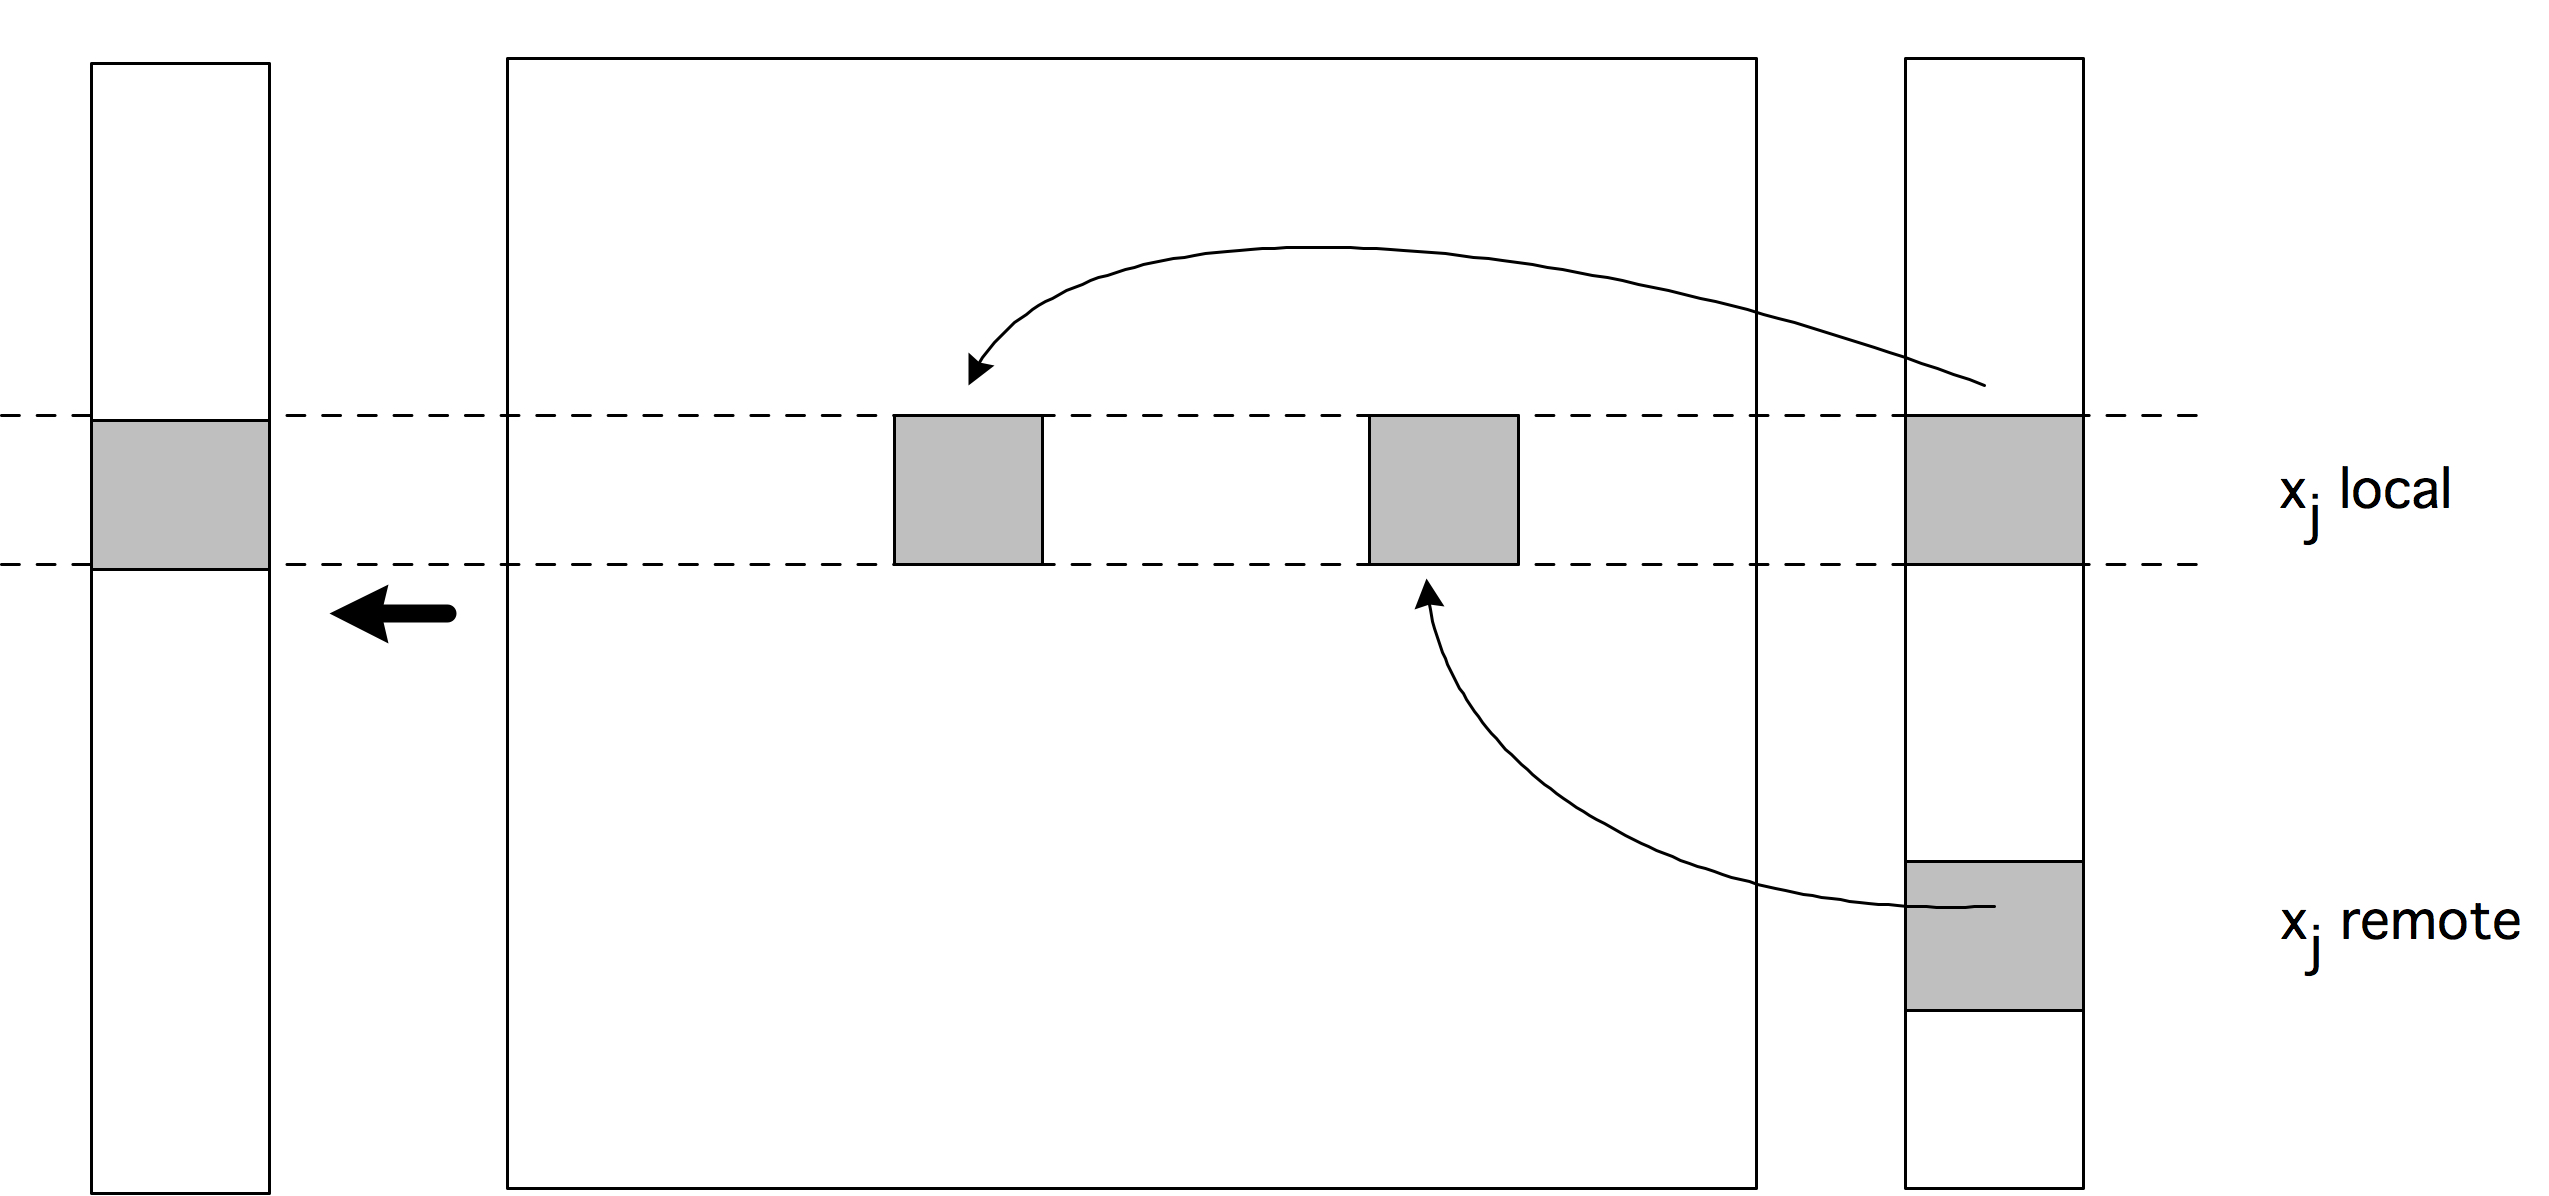
\includegraphics[scale=.12]{distmvp}
  \end{quote}
  \caption{The parallel matrix-vector product with a blockrow
    distribution.}
  \label{fig:distmvp}
\end{figure}
We can now proceed as follows:
\begin{itemize}
\item Start the transfer of non-local elements of~$x$;
\item Operate on the local elements of~$x$ while data transfer is
  going on;
\item Make sure that the transfers are finished;
\item Operate on the non-local elements of~$x$.
\end{itemize}

\begin{exercise}
  How much can you gain from overlapping computation and
  communication?  Hint: consider the border cases where computation
  takes zero time and and there is only communication, and the
  reverse. Now consider the general case.
\end{exercise}

Of course, this scenario presupposes that there is software and
hardware support for this overlap. MPI allows for this (see
section~\ref{sec:nonblocking}), through so-called
\indexterm{asynchronous communication} or \indexterm{non-blocking
  communication} routines. This does not immediately imply that
overlap will actually happen, since hardware support is an entirely
separate question.

